\documentclass[tikz, border=15pt]{standalone}
\usepackage{tikz}
\usetikzlibrary{calc, arrows.meta}

\definecolor{laserred}{HTML}{FF0000}
\definecolor{laserglow}{HTML}{FF8888}
\definecolor{mirrorcolor}{HTML}{A0AEC0}
\definecolor{glasscolor}{HTML}{E2E8F0}
\definecolor{screencolor}{HTML}{4A5568}

\begin{document}
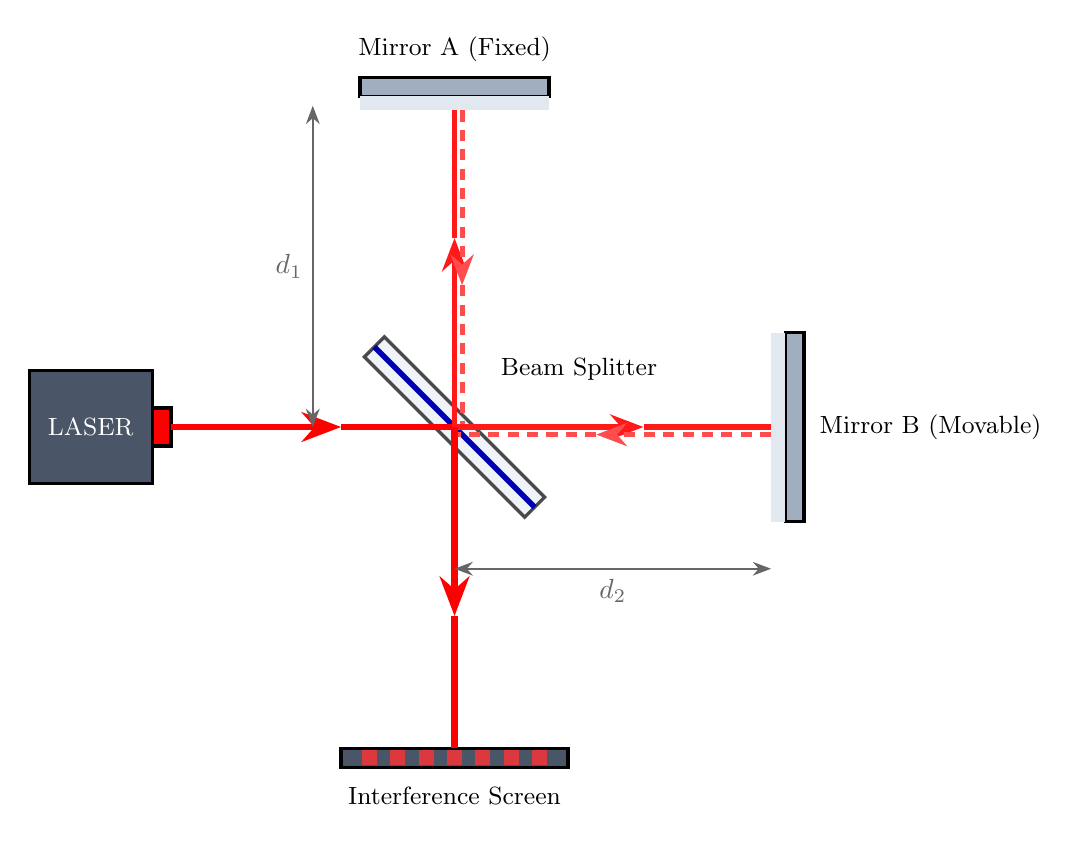
\begin{tikzpicture}[
    scale=1.2,
    >=Stealth,
    line width=1.2pt,
    font=\sffamily\bfseries
]

    % Grid alignment:
    % Laser source at (-4, 0)
    % Beam Splitter at (0, 0)
    % Mirror A (Fixed) at (0, 3.5)
    % Mirror B (Movable) at (3.5, 0)
    % Detector Screen at (0, -3.5)

    % 1. Laser Source
    \fill[screencolor, draw=black] (-4.5, -0.6) rectangle (-3.2, 0.6);
    \node[white, font=\small] at (-3.85, 0) {LASER};
    \fill[red, draw=black] (-3.2, -0.2) rectangle (-3.0, 0.2);

    % 2. Beam Splitter (at 45 degrees)
    \begin{scope}[rotate around={45:(0,0)}]
        \fill[glasscolor!80, draw=black, opacity=0.7] (-0.15, -1.2) rectangle (0.15, 1.2);
        % Semi-reflective coating line
        \draw[blue!70!black, line width=2pt] (0, -1.2) -- (0, 1.2);
    \end{scope}
    \node[above right=6pt, font=\small] at (0.2, 0.2) {Beam Splitter};

    % 3. Mirror A (Top - Arm 1)
    \fill[mirrorcolor, draw=black] (-1.0, 3.5) rectangle (1.0, 3.7);
    \fill[glasscolor] (-1.0, 3.35) rectangle (1.0, 3.5); % Front surface
    \node[above, font=\small] at (0, 3.75) {Mirror A (Fixed)};

    % 4. Mirror B (Right - Arm 2)
    \fill[mirrorcolor, draw=black] (3.5, -1.0) rectangle (3.7, 1.0);
    \fill[glasscolor] (3.35, -1.0) rectangle (3.5, 1.0); % Front surface
    \node[right, font=\small] at (3.75, 0) {Mirror B (Movable)};

    % 5. Screen / Detector (Bottom)
    \fill[screencolor, draw=black] (-1.2, -3.6) rectangle (1.2, -3.4);
    \node[below, font=\small] at (0, -3.7) {Interference Screen};
    % Fringe pattern simulation on screen
    \foreach \x in {-0.9, -0.6, -0.3, 0, 0.3, 0.6, 0.9} {
        \fill[laserred!80, opacity=0.8] (\x-0.08, -3.58) rectangle (\x+0.08, -3.42);
    }

    % Light Rays (Beams)
    % Incident Beam from Laser to BS
    \draw[->, line width=2.5pt, laserred] (-3.0, 0) -- (-1.2, 0);
    \draw[line width=2.5pt, laserred] (-1.2, 0) -- (0, 0);

    % Reflected Beam 1 (BS to Mirror A)
    \draw[->, line width=2pt, laserred!90] (0, 0) -- (0, 2.0);
    \draw[line width=2pt, laserred!90] (0, 2.0) -- (0, 3.35);

    % Return Beam 1 (Mirror A back to BS)
    \draw[->, line width=1.8pt, laserred!70, dash pattern=on 4pt off 3pt] (0.08, 3.35) -- (0.08, 1.5);
    \draw[line width=1.8pt, laserred!70, dash pattern=on 4pt off 3pt] (0.08, 1.5) -- (0.08, 0);

    % Transmitted Beam 2 (BS to Mirror B)
    \draw[->, line width=2pt, laserred!90] (0, 0) -- (2.0, 0);
    \draw[line width=2pt, laserred!90] (2.0, 0) -- (3.35, 0);

    % Return Beam 2 (Mirror B back to BS)
    \draw[->, line width=1.8pt, laserred!70, dash pattern=on 4pt off 3pt] (3.35, -0.08) -- (1.5, -0.08);
    \draw[line width=1.8pt, laserred!70, dash pattern=on 4pt off 3pt] (1.5, -0.08) -- (0, -0.08);

    % Recombined Beam (BS to Screen)
    \draw[->, line width=2.5pt, laserred] (0, 0) -- (0, -2.0);
    \draw[line width=2.5pt, laserred] (0, -2.0) -- (0, -3.4);

    % Arm Length Labels
    \draw[<->, line width=0.8pt, black!60] (-1.5, 0) -- (-1.5, 3.4) node[midway, left] {$d_1$};
    \draw[<->, line width=0.8pt, black!60] (0, -1.5) -- (3.35, -1.5) node[midway, below] {$d_2$};

\end{tikzpicture}
\end{document}
